\chapter{Franck-Hertz-Versuch}

<<<<<<< HEAD
\section{Aufbau}
% ---------------------------------------------------------------------------------------------
=======

\section{Theoretischer Hintergrund}
Der Franck-Hertz-Versuch, erstmals 1914 von James Franck und Gustav Hertz durchgeführt, lieferte den ersten direkten experimentellen Nachweis für quantisierte Energieniveaus in Atomen. Er bestätigte die entstehende Quantentheorie, indem er zeigte, dass Elektronen nur diskrete Energiemengen an Atome übertragen können, um diese in angeregte Zustände zu versetzen.
\vspace{0.3cm}\\
In diesem Versuch werden Elektronen durch eine glühende Kathode über Thermoemission freigesetzt und durch eine Beschleunigungsspannung $U_B$ durch mit Quecksilberdampf gefülltes Gas beschleunigt. Auf ihrem Weg durch das Gas können die Elektronen mit Quecksilberatomen zusammenstoßen. Abhängig von ihrer Energie verlaufen diese Stöße entweder elastisch oder inelastisch.
\vspace{0.3cm}\\
Solange die Elektronen nicht genügend kinetische Energie haben, um ein Atom anzuregen, finden nur elastische Stöße statt, bei denen die Elektronen nahezu keine Energie verlieren. Überschreiten sie jedoch die Anregungsenergie des Atoms, kommt es zu inelastischen Stößen, bei denen ein Elektron eine definierte Energiemenge an das Atom abgibt und dieses in einen angeregten Zustand überführt. Das Atom kehrt anschließend durch Emission eines Photons in den Grundzustand zurück, während das Elektron mit verminderter kinetischer Energie weiterfliegt.
\vspace{0.3cm}\\
Die niedrigste Anregungsenergie des Quecksilberatoms liegt bei etwa
\begin{equation}
\Delta E \approx \SI{4.67}{\electronvolt} 
\end{equation}
und entspricht dem Übergang vom Grundzustand $6^1S_0$ in den angeregten Zustand $6^3P_1$ \cite{Hg_excitationEnergy}.
\vspace{0.3cm}\\
Bevor die Elektronen die Anode erreichen, müssen sie eine kleine Gegenspannung $U_G$ überwinden. Elektronen, die durch inelastische Stöße zu viel Energie verlieren, können diese Barriere nicht überwinden und tragen daher nicht zum gemessenen Anodenstrom $I_A$ bei.
\vspace{0.3cm}\\
Wenn die Beschleunigungsspannung $U_B$ schrittweise erhöht wird, steigt der Anodenstrom zunächst an, da mehr Elektronen die Anode erreichen. Sobald $e U_B \geq \SI{4.67}{\electronvolt}$ ist, beginnen inelastische Stöße $\rightarrow$ einige Elektronen verlieren Energie $\rightarrow$ weniger Elektronen überwinden $U_G$ $\rightarrow$ $I_A$ sinkt. Mit weiter steigender Spannung gewinnen die Elektronen erneut genug Energie $\rightarrow$ $I_A$ steigt wieder, bis eine zweite Anregung möglich wird $\rightarrow$ zweites Minimum. So entsteht eine periodische Folge von Maxima und Minima im Strom-Spannungs-Diagramm.
\vspace{0.3cm}\\
Der Abstand zwischen zwei benachbarten Maxima oder Minima entspricht der Anregungsenergie:
\begin{equation}
\Delta E = e \cdot \Delta U
\end{equation}
\vspace{0.3cm}\\
Die kinetische Energie der Elektronen ergibt sich aus:
\begin{equation}
E_{\text{kin}} = e \cdot U_B
\end{equation}
\vspace{0.3cm}\\
Die Temperatur beeinflusst über den Dampfdruck die mittlere freie Weglänge der Elektronen. Ein höherer Dampfdruck (bei höherer Temperatur) führt zu häufigeren Stößen, wodurch die Maxima in der Stromkurve unschärfer werden. Ist die Temperatur zu niedrig, finden kaum Stöße statt und es erscheint keine Struktur im Stromverlauf.
\vspace{0.3cm}\\
Die mittlere freie Weglänge $\lambda$ lässt sich näherungsweise berechnen durch:
\begin{equation}
\lambda = \frac{k_B T}{\sqrt{2} \pi d^2 p}
\end{equation}
mit $k_B$ als Boltzmann-Konstante, $T$ der Temperatur, $d$ dem Atomdurchmesser und $p$ dem Dampfdruck.
\vspace{0.3cm}\\
Die Gegenspannung $U_G$ wirkt als Filter für langsame Elektronen. Eine Erhöhung von $U_G$ reduziert den gemessenen Strom, verändert jedoch nicht die Lage der Maxima.
\vspace{0.3cm}\\
Der Franck-Hertz-Versuch stellt einen Meilenstein der Atomphysik dar. Er zeigte experimentell, dass Energieübertragungen zwischen Elektronen und Atomen in diskreten Beträgen erfolgen und bestätigte die Annahmen des Bohrschen Atommodells.

\section{Aufbau}

\begin{figure}[H]
    \centering
    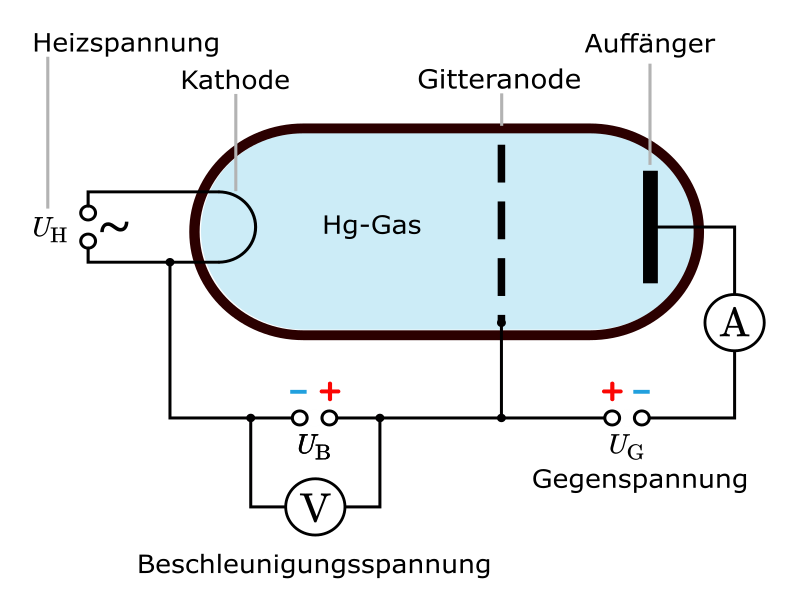
\includegraphics[width=0.5\textwidth]{FranckHertz.png}
    \caption{Franck-Hertz-Schaltung \cite{FranckHertzHg}} 
    \label{fig:FrankHertzSchaltung}    
\end{figure}

Der experimentelle Aufbau (schematisch in \cref{fig:FrankHertzSchaltung}) besteht aus einer mit Quecksilberdampf (Hg-Gas) gefüllten Franck-Hertz-Röhre, die sich in einem temperaturgeregelten Ofen befindet. Elektronen werden durch Glühemission aus einer beheizten Kathode freigesetzt und mit einer einstellbaren Beschleunigungsspannung $ U_B $ in Richtung eines Gitters beschleunigt. Nach dem Passieren des Gitters stoßen die Elektronen auf eine kleine Gegenspannung $ U_G $, bevor sie die Anode erreichen.
\vspace{0.3cm}\\
Die Gegenspannung $ U_G $ stellt sicher, dass nur Elektronen mit ausreichend kinetischer Energie - also solche, die keine oder nur elastische Stöße erfahren haben - die Anode erreichen können. Der resultierende Anodenstrom $ I_A $ wird mit einem empfindlichen Amperemeter gemessen. Die Beschleunigungsspannung $ U_B $ wird mit einem Voltmeter überwacht.
\vspace{0.3cm}\\
Der Ofen ermöglicht die präzise Temperaturregelung des Quecksilberdampfes, was entscheidend ist, da die Dampfdruckabhängigkeit die mittlere freie Weglänge der Elektronen beeinflusst. Eine konstante Temperatur ist notwendig, um reproduzierbare und deutlich sichtbare Maxima in der Franck-Hertz-Kurve zu erhalten.
\vspace{0.3cm}\\
Die gesamte Apparatur wird über eine externe Steuereinheit betrieben, die das automatische Hochfahren der Beschleunigungsspannung sowie eine synchrone Datenaufnahme über die Messsoftware erlaubt.
\vspace{0.3cm}\\
% ----------------------------------------------------------------------------------
% ----------------------------------------------------------------------------------

>>>>>>> ppg
\subsection{Subsection}
% ---------------------------------------------------------------------------------------------
\subsubsection{Subsubsection}
